

\tikzset{every picture/.style={line width=0.75pt}} %set default line width to 0.75pt        

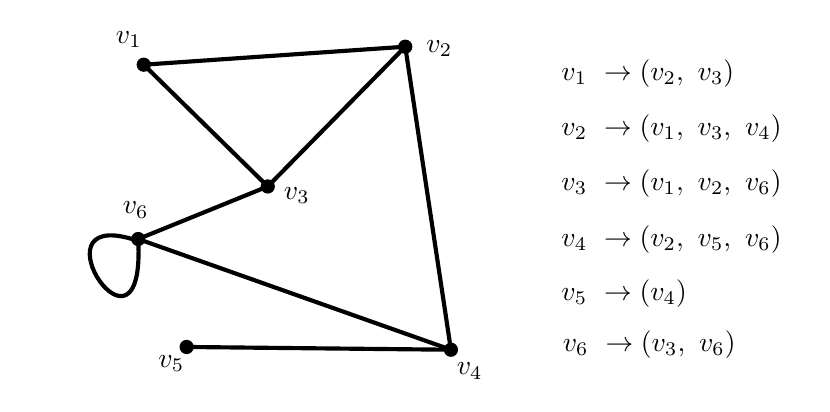
\begin{tikzpicture}[x=0.5pt,y=0.5pt,yscale=-1,xscale=1]
%uncomment if require: \path (0,285); %set diagram left start at 0, and has height of 285

%Flowchart: Connector [id:dp8969448059697392] 
\draw  [fill={rgb, 255:red, 0; green, 0; blue, 0 }  ,fill opacity=1 ] (64,41) .. controls (64,38.58) and (65.96,36.62) .. (68.38,36.62) .. controls (70.79,36.62) and (72.75,38.58) .. (72.75,41) .. controls (72.75,43.42) and (70.79,45.38) .. (68.38,45.38) .. controls (65.96,45.38) and (64,43.42) .. (64,41) -- cycle ;
%Flowchart: Connector [id:dp7390561295523319] 
\draw  [fill={rgb, 255:red, 0; green, 0; blue, 0 }  ,fill opacity=1 ] (253,28) .. controls (253,25.58) and (254.96,23.62) .. (257.38,23.62) .. controls (259.79,23.62) and (261.75,25.58) .. (261.75,28) .. controls (261.75,30.42) and (259.79,32.38) .. (257.38,32.38) .. controls (254.96,32.38) and (253,30.42) .. (253,28) -- cycle ;
%Flowchart: Connector [id:dp17940799737904434] 
\draw  [fill={rgb, 255:red, 0; green, 0; blue, 0 }  ,fill opacity=1 ] (286,247) .. controls (286,244.58) and (287.96,242.62) .. (290.38,242.62) .. controls (292.79,242.62) and (294.75,244.58) .. (294.75,247) .. controls (294.75,249.42) and (292.79,251.38) .. (290.38,251.38) .. controls (287.96,251.38) and (286,249.42) .. (286,247) -- cycle ;
%Flowchart: Connector [id:dp3782169610007916] 
\draw  [fill={rgb, 255:red, 0; green, 0; blue, 0 }  ,fill opacity=1 ] (95,245) .. controls (95,242.58) and (96.96,240.62) .. (99.38,240.62) .. controls (101.79,240.62) and (103.75,242.58) .. (103.75,245) .. controls (103.75,247.42) and (101.79,249.38) .. (99.38,249.38) .. controls (96.96,249.38) and (95,247.42) .. (95,245) -- cycle ;
%Straight Lines [id:da4623211688485681] 
\draw [color={rgb, 255:red, 0; green, 0; blue, 0 }  ,draw opacity=1 ][line width=1.5]    (68.38,41) -- (257.38,28) ;
%Flowchart: Connector [id:dp9777596548306114] 
\draw  [fill={rgb, 255:red, 0; green, 0; blue, 0 }  ,fill opacity=1 ] (153.62,129) .. controls (153.62,126.58) and (155.58,124.62) .. (158,124.62) .. controls (160.42,124.62) and (162.38,126.58) .. (162.38,129) .. controls (162.38,131.42) and (160.42,133.38) .. (158,133.38) .. controls (155.58,133.38) and (153.62,131.42) .. (153.62,129) -- cycle ;
%Straight Lines [id:da48210138973948524] 
\draw [color={rgb, 255:red, 0; green, 0; blue, 0 }  ,draw opacity=1 ][line width=1.5]    (158,129) -- (257.38,28) ;
%Straight Lines [id:da8804269357524794] 
\draw [color={rgb, 255:red, 0; green, 0; blue, 0 }  ,draw opacity=1 ][line width=1.5]    (99.38,245) -- (290.38,247) ;
%Straight Lines [id:da7237087103773605] 
\draw [color={rgb, 255:red, 0; green, 0; blue, 0 }  ,draw opacity=1 ][line width=1.5]    (290.38,247) -- (257.38,28) ;
%Straight Lines [id:da1730143543571403] 
\draw [color={rgb, 255:red, 0; green, 0; blue, 0 }  ,draw opacity=1 ][line width=1.5]    (64.38,167) -- (158,129) ;
%Flowchart: Connector [id:dp14114310861231993] 
\draw  [fill={rgb, 255:red, 0; green, 0; blue, 0 }  ,fill opacity=1 ] (60,167) .. controls (60,164.58) and (61.96,162.62) .. (64.38,162.62) .. controls (66.79,162.62) and (68.75,164.58) .. (68.75,167) .. controls (68.75,169.42) and (66.79,171.38) .. (64.38,171.38) .. controls (61.96,171.38) and (60,169.42) .. (60,167) -- cycle ;
%Curve Lines [id:da28133541410560436] 
\draw [line width=1.5]    (64.38,167) .. controls (70,270) and (-14,145) .. (60,167) ;
%Straight Lines [id:da19428173586433062] 
\draw [color={rgb, 255:red, 0; green, 0; blue, 0 }  ,draw opacity=1 ][line width=1.5]    (290.38,247) -- (64.38,167) ;
%Straight Lines [id:da22211986944091267] 
\draw [color={rgb, 255:red, 0; green, 0; blue, 0 }  ,draw opacity=1 ][line width=1.5]    (158,129) -- (68.38,41) ;

% Text Node
\draw (46,15) node [anchor=north west][inner sep=0.75pt]   [align=left] {$\displaystyle v_{1}$};
% Text Node
\draw (167.38,127.38) node [anchor=north west][inner sep=0.75pt]   [align=left] {$\displaystyle v_{3}$};
% Text Node
\draw (76.75,249) node [anchor=north west][inner sep=0.75pt]   [align=left] {$\displaystyle v_{5}$};
% Text Node
\draw (292.38,254.38) node [anchor=north west][inner sep=0.75pt]   [align=left] {$\displaystyle v_{4}$};
% Text Node
\draw (270.38,21.38) node [anchor=north west][inner sep=0.75pt]   [align=left] {$\displaystyle v_{2}$};
% Text Node
\draw (368,35.09) node [anchor=north west][inner sep=0.75pt]   [align=left] {$\displaystyle v_{1} \ \rightarrow ( v_{2} ,\ v_{3})$};
% Text Node
\draw (368,74.84) node [anchor=north west][inner sep=0.75pt]   [align=left] {$\displaystyle v_{2} \ \rightarrow ( v_{1} ,\ v_{3} ,\ v_{4})$};
% Text Node
\draw (368,114.59) node [anchor=north west][inner sep=0.75pt]   [align=left] {$\displaystyle v_{3} \ \rightarrow ( v_{1} ,\ v_{2} ,\ v_{6})$};
% Text Node
\draw (368,155.34) node [anchor=north west][inner sep=0.75pt]   [align=left] {$\displaystyle v_{4} \ \rightarrow ( v_{2} ,\ v_{5} ,\ v_{6})$ \ };
% Text Node
\draw (368,194.09) node [anchor=north west][inner sep=0.75pt]   [align=left] {$\displaystyle v_{5} \ \rightarrow ( v_{4})$};
% Text Node
\draw (51,138) node [anchor=north west][inner sep=0.75pt]   [align=left] {$\displaystyle v_{6}$};
% Text Node
\draw (369,231.09) node [anchor=north west][inner sep=0.75pt]   [align=left] {$\displaystyle v_{6} \ \rightarrow ( v_{3} ,\ v_{6})$};


\end{tikzpicture}

